\documentclass[conference]{assets/latex/IEEEtran}

\usepackage{amsmath,amssymb,amsfonts}
\usepackage{graphicx}
\usepackage{textcomp}
\usepackage{xcolor}
\usepackage[backend=biber,style=numeric]{biblatex}
\addbibresource{assets/latex/report.bib}

\graphicspath{{assets/latex/}}

\begin{document}

\title{CS6524 Computer Vision Lab. 3\\ Structure from Motion}

\author{\IEEEauthorblockN{Dara Heaphy}
\IEEEauthorblockA{\textit{Student ID 23369914} \\
University of Limerick\\
Limerick, Ireland \\
23369914@studentmail.ul.ie}
}

\maketitle

\begin{abstract}
I reconstructed a desk globe from two phone videos: one where I walk the
camera around it ($a$) and one where I spin it by hand ($b$). For $a$ the
camera path closes a full $362^\circ$ circle and I get a dense cap of the
globe. Video $b$ didn't work in any of the six runs. Getting the focal length
wrong or skipping undistortion mostly hurts by making one frame fail to
register, and after that the whole path goes off.
\end{abstract}

% =====================================================================
\section{Introduction}
Structure from motion is stereo with $N$ frames instead of two. From one
camera moving around an object you have to work out where the camera was in
every frame and where the points are in 3D, both at the same time, and up to
an unknown scale. I used the calibration from lab2, built a sequential
pipeline (match, essential matrix, PnP, bundle adjustment), turned it into a
dense point cloud, and then re-ran it with the focal length scaled by 0.8 and
1.2, with and without undistortion.

% =====================================================================
\section{Methodology}

\subsection{Data}
Same iPhone as lab2 (1080$\times$1920, 30\,fps). I resize every frame to
360$\times$640 in exactly the same way as the lab2 calibration video, so $K$
and $D$ still apply, and keep every second frame (15\,fps) to get the files
under 5\,MB. The object is a globe on a stand, on a grey rug over a wooden
floor. The room was quite dark, which ended up mattering a lot.

\subsection{Masking}
In $b$ the camera is still and the globe turns, so the background is not part
of the same rigid scene. If I let features from the rug into $b$, they would
say the camera didn't move. I segment the globe by colour. I measured the HSV
hue of each part: floor and rug 12--17, skin 7--11, land 18--58, ocean
75--120. So the biggest saturated blob with hue $\ge 19$, with holes filled,
is the globe, and the hand drops out too. My first try, the largest ocean
blob only, missed the globe whenever the Asia side faced the camera. In $a$
everything is static, so there I use the whole frame for features (the rug
helps the pose a lot) and only use the mask for the dense step.

\subsection{Features and keyframes}
I use SIFT with CLAHE on the grey image because of the low light, Lowe's
ratio test (0.8), a mutual-match check, and a RANSAC essential matrix (1\,px)
to throw out bad matches. I also compared ORB and AKAZE on 29 globe-only
frame pairs. ORB actually found more inliers (median 465 vs 169 for SIFT in
$a$), but in two full runs on $b$ it had 15 and 17 PnP failures against 2--4
for SIFT, so its extra matches don't last long enough to be useful.

A fixed frame step didn't work for $b$, because I turned the globe in bursts
(up to $7^\circ$ per frame) with pauses in between to re-grip it. Instead a
frame becomes the next keyframe once the matches have moved 20\,px on
average, or just before too few matches would be left.

\subsection{Camera poses}
For every pair of neighbouring keyframes I estimate $E$ and get $R$ and $t$
from it. I triangulate the matches with the first camera at the origin and
reproject them into both frames; that's the two-view error in
Table~\ref{tab:sens}.

Just chaining these pairs doesn't work, because each $t$ has length 1, so the
scale is different for every pair. So I start from the first pair with enough
parallax, then add each new keyframe with \texttt{solvePnPRansac} against the
3D points I already have, which keeps one scale throughout. New points are
triangulated between the first and the current frame that sees them, if the
rays are at least $1^\circ$ apart ($0.5^\circ$ in $b$). Every 5 keyframes I run
bundle adjustment over the last 10 cameras, with the older cameras held fixed
so the scale stays put, and at the end one global bundle adjustment
(\texttt{scipy least\_squares}, Huber loss). If PnP fails, I fall back to the
pair's $E$ with the previous step length.

My first version broke right at the start of $a$. I barely moved the phone in
the first second, so $E$ came out as a $180^\circ$ rotation and every match
was rejected, which cut every track. Building the tracks from the RANSAC
inliers of $E$ instead of the \texttt{recoverPose} mask fixed it.

\subsection{Dense cloud}
For each keyframe and the one two after it I compute DIS optical flow both
ways and keep pixels in the mask where going there and back lands within
0.5\,px. I triangulate those pixels with the known cameras and keep them if
they reproject within 1\,px and the rays are at least $4^\circ$ apart. All the
points go into a voxel grid where each voxel takes the average position and
colour, and I drop voxels that only one pair saw. For $b$ I had to loosen
this, or nothing was left.

\subsection{How I measured it}
There is no ground truth, so I use three checks. Both videos do one full
turn and end where they started, so the camera path should sweep about
$360^\circ$ and the gap between the first and last camera, divided by the
radius of the path, should be about 0. And the globe is a sphere, so I fit a
sphere to the dense cloud and report the error as a percentage of its
radius.

% =====================================================================
\section{Results}
Table~\ref{tab:sens} has all twelve runs and Fig.~\ref{fig:overview} the two
main ones. For $a$ the path closes: it sweeps $362^\circ$ with a gap of
$0.17R$, and bundle adjustment brings the error from 0.42 to 0.35\,px over
about 30k points. The dense cloud is the top half of the globe, with the knob
on top visible. I never filmed below the equator, so the bottom isn't there.
The sphere error is 4.6\%, partly because bits of the metal ring and the
stand get through the mask.

\begin{table}[t]
\caption{All runs. kf: keyframes used/selected; 2-view: two-view
reprojection error; BA: error before $\to$ after global bundle adjustment;
swept: angle of the camera path (should be $360^\circ$); gap: start--end
gap over path radius (should be 0); sphere: sphere-fit error.}
\label{tab:sens}
\centering\scriptsize\setlength{\tabcolsep}{3pt}
\begin{tabular}{@{}lrrrrrrr@{}}
\hline
run & kf & 2-view & BA & swept & gap & sphere & dense \\
 & reg. & px & px & deg & $/R$ & \% & pts \\
\hline
a\_08u & 54/54 & 0.24 & 0.94$\to$0.54 & 165 & 2.13 & 6.0 & 972 \\
a\_10u & 53/53 & 0.23 & 0.42$\to$0.35 & 362 & 0.17 & 4.6 & 30558 \\
a\_12u & 54/54 & 0.22 & 0.33$\to$0.29 & 384 & 0.49 & 4.8 & 29982 \\
a\_08d & 54/54 & 0.23 & 1.01$\to$0.61 & 72 & 1.55 & 4.3 & 6217 \\
a\_10d & 54/54 & 0.23 & 1.45$\to$0.52 & 184 & 1.91 & 4.3 & 8288 \\
a\_12d & 54/54 & 0.22 & 0.37$\to$0.32 & 366 & 0.27 & 3.9 & 23799 \\
\hline
b\_08u & 38/38 & 0.22 & 0.65$\to$0.47 & 299 & 0.96 & 8.6 & 220130 \\
b\_10u & 37/37 & 0.22 & 1.05$\to$0.46 & 121 & 1.59 & 8.5 & 197533 \\
b\_12u & 38/38 & 0.23 & 1.01$\to$0.50 & 197 & 1.88 & 5.6 & 109938 \\
b\_08d & 38/38 & 0.22 & 1.25$\to$0.42 & 161 & 1.56 & 7.9 & 227246 \\
b\_10d & 38/38 & 0.22 & 0.68$\to$0.32 & 209 & 1.37 & 7.9 & 215986 \\
b\_12d & 36/38 & 0.23 & 0.72$\to$0.30 & 148 & 1.82 & 6.5 & 63305 \\
\hline
\end{tabular}

\end{table}

\begin{figure}[t]
\centerline{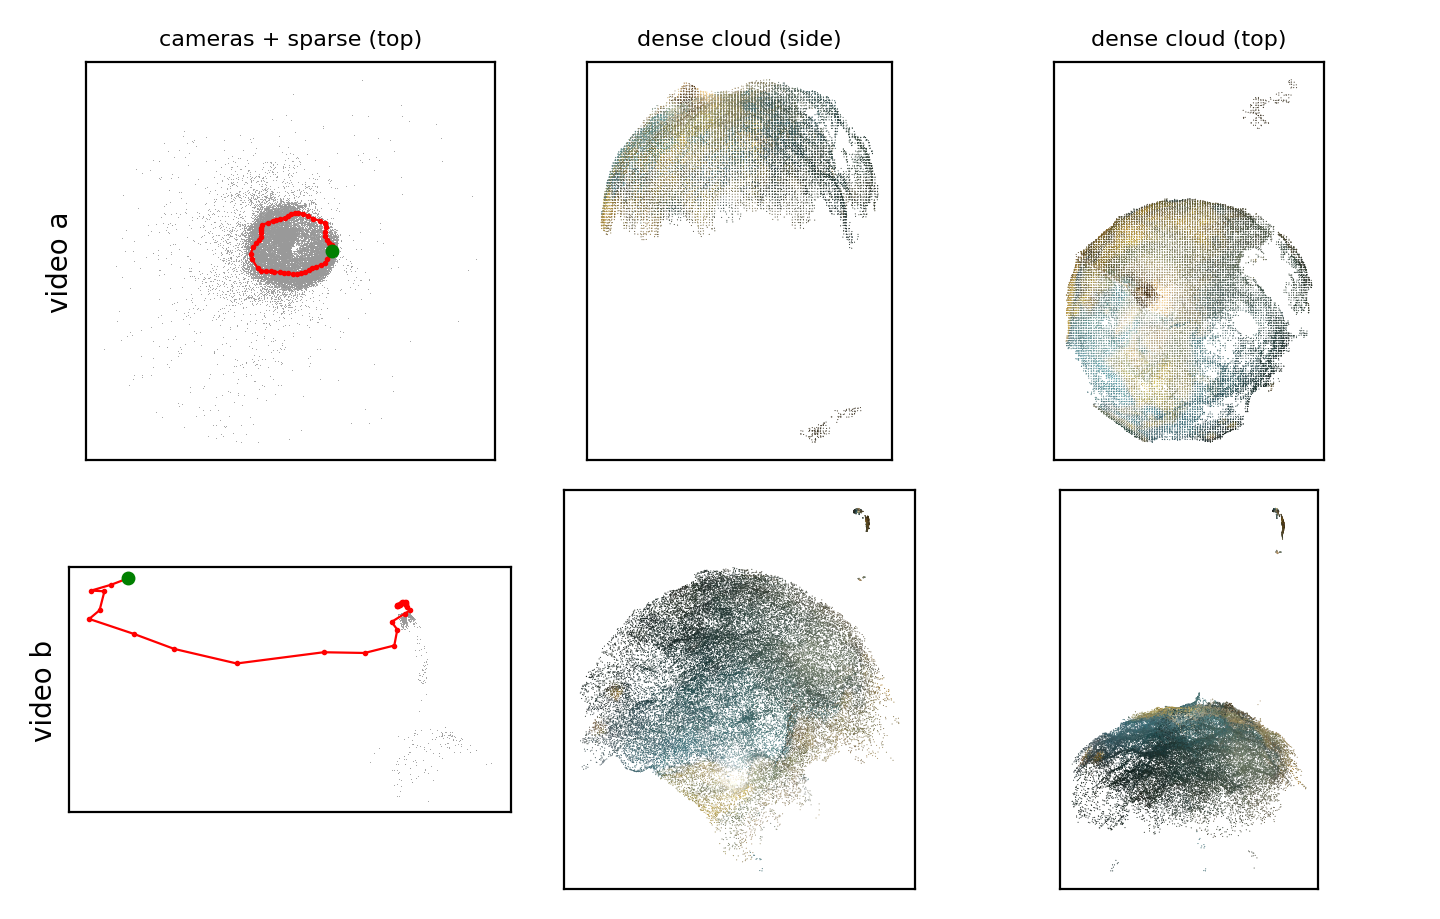
\includegraphics[width=\columnwidth]{overview.png}}
\caption{Top: $a$, bottom: $b$, both at $f{\times}1$, undistorted. Left:
camera path from above (green is the start) over the sparse points. Middle
and right: dense cloud from the side and from above.}
\label{fig:overview}
\end{figure}

\begin{figure}[t]
\centerline{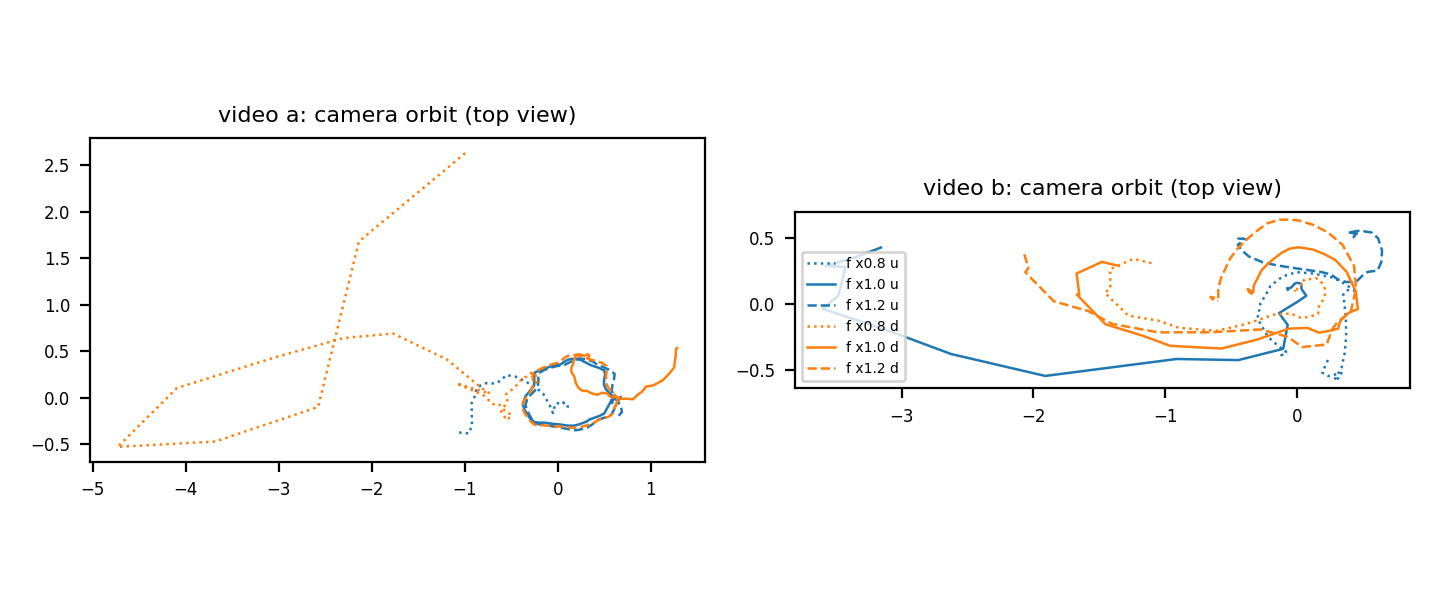
\includegraphics[width=\columnwidth]{orbits.png}}
\caption{Camera paths from above for all six runs of each video. Blue:
undistorted, orange: not. Dotted, solid, dashed: $f\times0.8$, 1, 1.2.}
\label{fig:orbits}
\end{figure}

\textbf{Focal length.} With $f\times1.2$ the path still closes, but it sweeps
$384^\circ$ and the gap triples to $0.49R$. With $f\times0.8$ the error
before global BA doubles (0.94 vs 0.42\,px), two frames fail PnP, and the path
breaks after $165^\circ$; the dense cloud drops to 972 points because the pairs
no longer agree. What surprised me is that the final error is lowest at
$f\times1.2$ (0.29\,px). So reprojection error can't tell you the focal length
is wrong, but the loop gap can, and it picks the calibrated value.

\textbf{Distortion.} The lab2 distortion moves pixels by only 0.25\,px
(median) in the middle of the image, where the globe is, but up to 26\,px in
the corners. In $a$ the features come from the whole frame, so without
undistortion the error before BA goes from 0.42 to 1.45\,px and the path
breaks at $184^\circ$. But $a\_12d$ closes anyway ($366^\circ$), so it isn't a
simple steady effect.

\textbf{Video $b$} didn't work in any run: the paths sweep 121--$299^\circ$ and
the gaps are all $0.96R$ or more (Fig.~\ref{fig:orbits}). The odd part is
that its reprojection errors (0.30--0.50\,px) are as low as $a$'s. Each short
stretch of the path is consistent, but the stretches don't add up to a
circle. The dense clouds still look like a globe, but they are several
shells that don't line up (5.6--8.6\% sphere error).

% =====================================================================
\section{Discussion and Failure Analysis}
\textbf{It either works or it doesn't.} The clearest thing in
Table~\ref{tab:sens}: the three runs with no PnP failures ($a\_10u$,
$a\_12u$, $a\_12d$) all close the loop, and every run with at least one
failure doesn't. When PnP fails, the fallback uses $E$ with a guessed step
length, which is wrong, and the windowed bundle adjustment can't fix it
because the cameras before the window are fixed. So a wrong $K$ or $D$
doesn't slowly bend a good path. It pushes a weak part of the video over the
edge.

\textbf{Why $b$ fails.} It only gets about 140 inliers per pair against about
1000 in $a$, because I had to mask out the background and the globe is dark
and half in shadow. My hand covers a lot of the globe while it turns it, the
turning comes in bursts, and the tracks only last about 2.6 keyframes. I was
also holding the phone, so the motion isn't a clean spin about one axis. ORB
made it worse, so the problem is how long the tracks last, not how many
matches there are.

\textbf{A second attempt.} I also filmed a second pair (a pink cup with a toy
lion on it, in brighter light) to see if a different object would help. It
was worse: $a$ didn't close in any run ($157^\circ$ at $f\times1$). The
frame-to-frame rotations added up to $347^\circ$, but the steps between
cameras shrank to almost nothing, so the path turned into the camera rotating
on the spot. I was further away, so the far floor and wall dominated, and
those points barely move between frames. The cup is also mostly plain
plastic, which gave $b$ only about 75 inliers per pair. So I kept the globe
videos.

\textbf{What I'd do next.} Add loop closure (match the last frames to the
first and put them into the final bundle adjustment), since both videos end
where they started. For $b$, use the fact that it's a turntable: one axis and
one angle per frame instead of a full pose. Re-film $b$ on a tripod with more
light and a slow, steady spin without my hand on the globe. When PnP fails,
try matching against all earlier keyframes instead of falling back to $E$.
For the dense step, use more than two views at once.

% =====================================================================
\section{Conclusion}
The pipeline reconstructs the globe from the orbit video with the path
closing to within 0.17 of its radius, but fails on the spinning video. What I
learned: one bad registration ruins the whole path, low reprojection error
doesn't mean the result is right, and filming (light, distance, texture, a
steady motion) matters more than any parameter I changed.

\nocite{foundationsCVbook}
\printbibliography

\end{document}
